\section{System dialogów w grach (Bartosz Strzelecki)}\label{chap:dialogi}
Systemy dialogów w grach wideo kształtują wciągającą historię, umożliwiając graczom dokonywanie wyborów, które wpływają na relacje między postaciami, zadania i narrację gry. 
Odkrywają wiedzę, pogłębiają zaangażowanie i oferują dynamiczną rozgrywkę poprzez różnorodne podejmowanie decyzji.
Dialogi umożliwiają graczowi wpłynięcie na świat, pozwalając mu wybrać, w którą stronę historia będzie podążać.
Gracz w ten sposób rozwiązuje dylematy moralne i może wczuć się w klimat rozgrywki.
"Najpopularniejsze zachodnie gry RPG, takie jak serie Baldur's Gate i Fallout, żyją i umierają dzięki sile dialogów i zdolności gracza do wpływania na postacie niezależne." \cite{dialogue}.

W \textit{Mass Effect 3}\footnote{\url{https://www.ea.com/games/mass-effect/mass-effect-3}} system dialogowy jest integralną częścią rozgrywki i pozwala graczom na prowadzenie rozmów z różnymi postaciami w trakcie gry.
System dialogów w \textit{Mass Effect 3} wykorzystuje interfejs oparty na kole dialogowym (rys. \ref{fig:wheel}), które
przedstawia graczom wiele opcji odpowiedzi podczas rozmów, zwykle podzielonych na kategorie według ich ogólnego tonu lub intencji.
Dostępne opcje często obejmują wybory dyplomatyczne, agresywne bądź konfrontacyjne oraz opcje neutralne lub śledcze.
Podczas niektórych rozmów lub przerywników filmowych gracze mogą przerwać trwającą rozmowę, szybko wybierając określoną opcję dialogową.
Te opcje przerywania pozwalają graczom podjąć natychmiastowe działania lub podjąć decyzje na miejscu, często wpływając na wynik sytuacji lub relacje postaci z innymi.
Ogólnie rzecz biorąc, system dialogowy w \textit{Mass Effect 3} został zaprojektowany tak, aby zapewnić graczom bogate i wciągające doświadczenie w opowiadaniu historii,
pozwalając im kształtować narrację poprzez wybory i interakcje z olbrzymią gamą postaci. System oferuje różnorodne opcje odpowiedzi, dynamiczne rozmowy i konsekwencje,
przyczyniając się do fascynującej i rozgałęzionej narracji gry.

Alternatywnym rozwiązaniem jest to zaprezentowane w grze \textit{Fallout 3}\footnote{\url{https://fallout.bethesda.net/pl}} (rys. \ref{fig:fallout}), które odróżniają przede wszystkim możliwe odpowiedzi gracza.
W tym przypadku użytkownik wybiera z listy gotową odpowiedź, zamiast jedynie tonu jak w grze \textit{Mass Effect}. Pozwala to na większą kontrolę
przez gracza oraz umożliwia uniknięcie sytuacji, w której gracz spodziewał się innej odpowiedzi, wybierając daną opcję dialogową.

\begin{figure}[h]
\centering
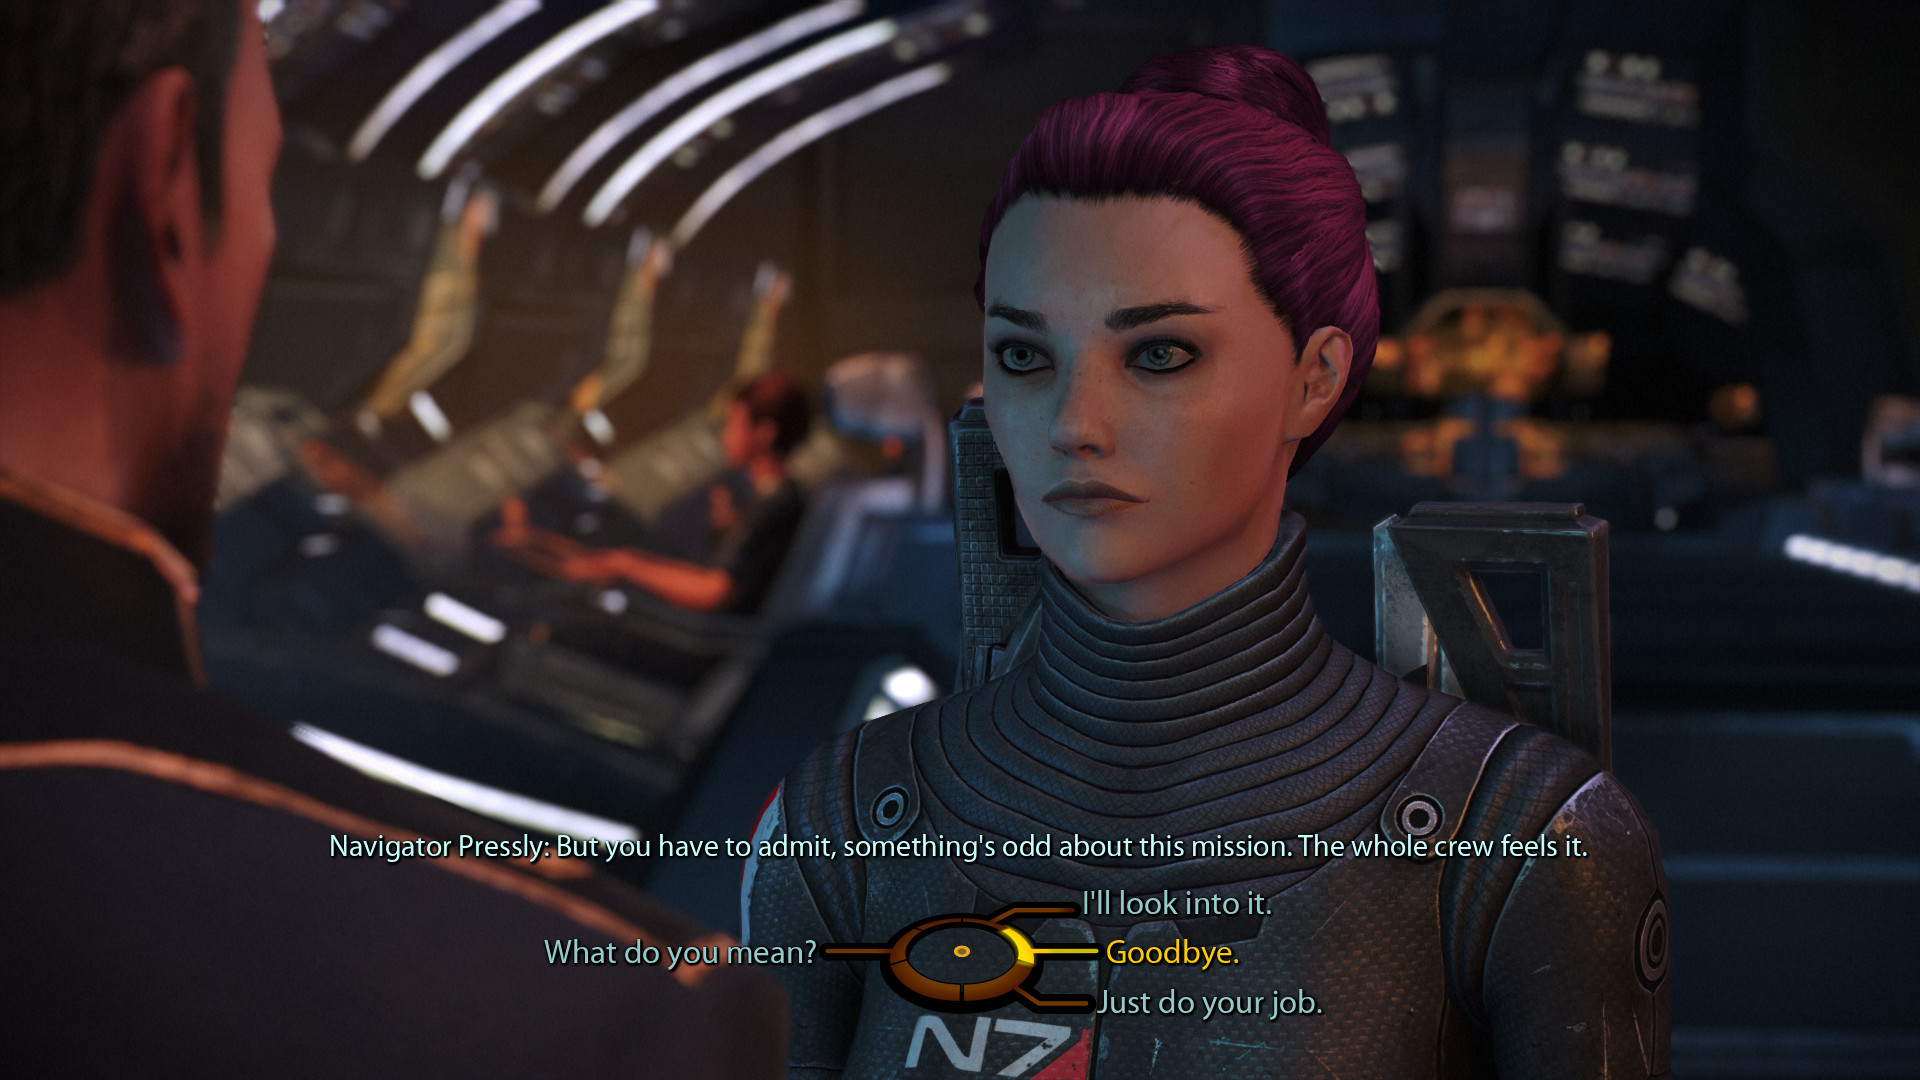
\includegraphics[width=0.8\textwidth]{images/me}
\caption[Przykład koła dialogowego w grze \textit{Mass Effect}.]{Przykład koła dialogowego w grze \textit{Mass Effect}\protect\footnotemark.}
\label{fig:wheel}
\end{figure}
\footnotetext{Internet, \url{https://cdn.vox-cdn.com/thumbor/DP9qp4fQbE88gJMar2WlwAJ1gRg=/0x0:1920x1080/920x0/filters:focal(0x0:1920x1080):format(webp):no_upscale()/cdn.vox-cdn.com/uploads/chorus_asset/file/22515161/5_14_2021_10_51_45_AM_5044r2pc.png}, dostęp: 12.09.2023}

\begin{figure}[h]
\centering
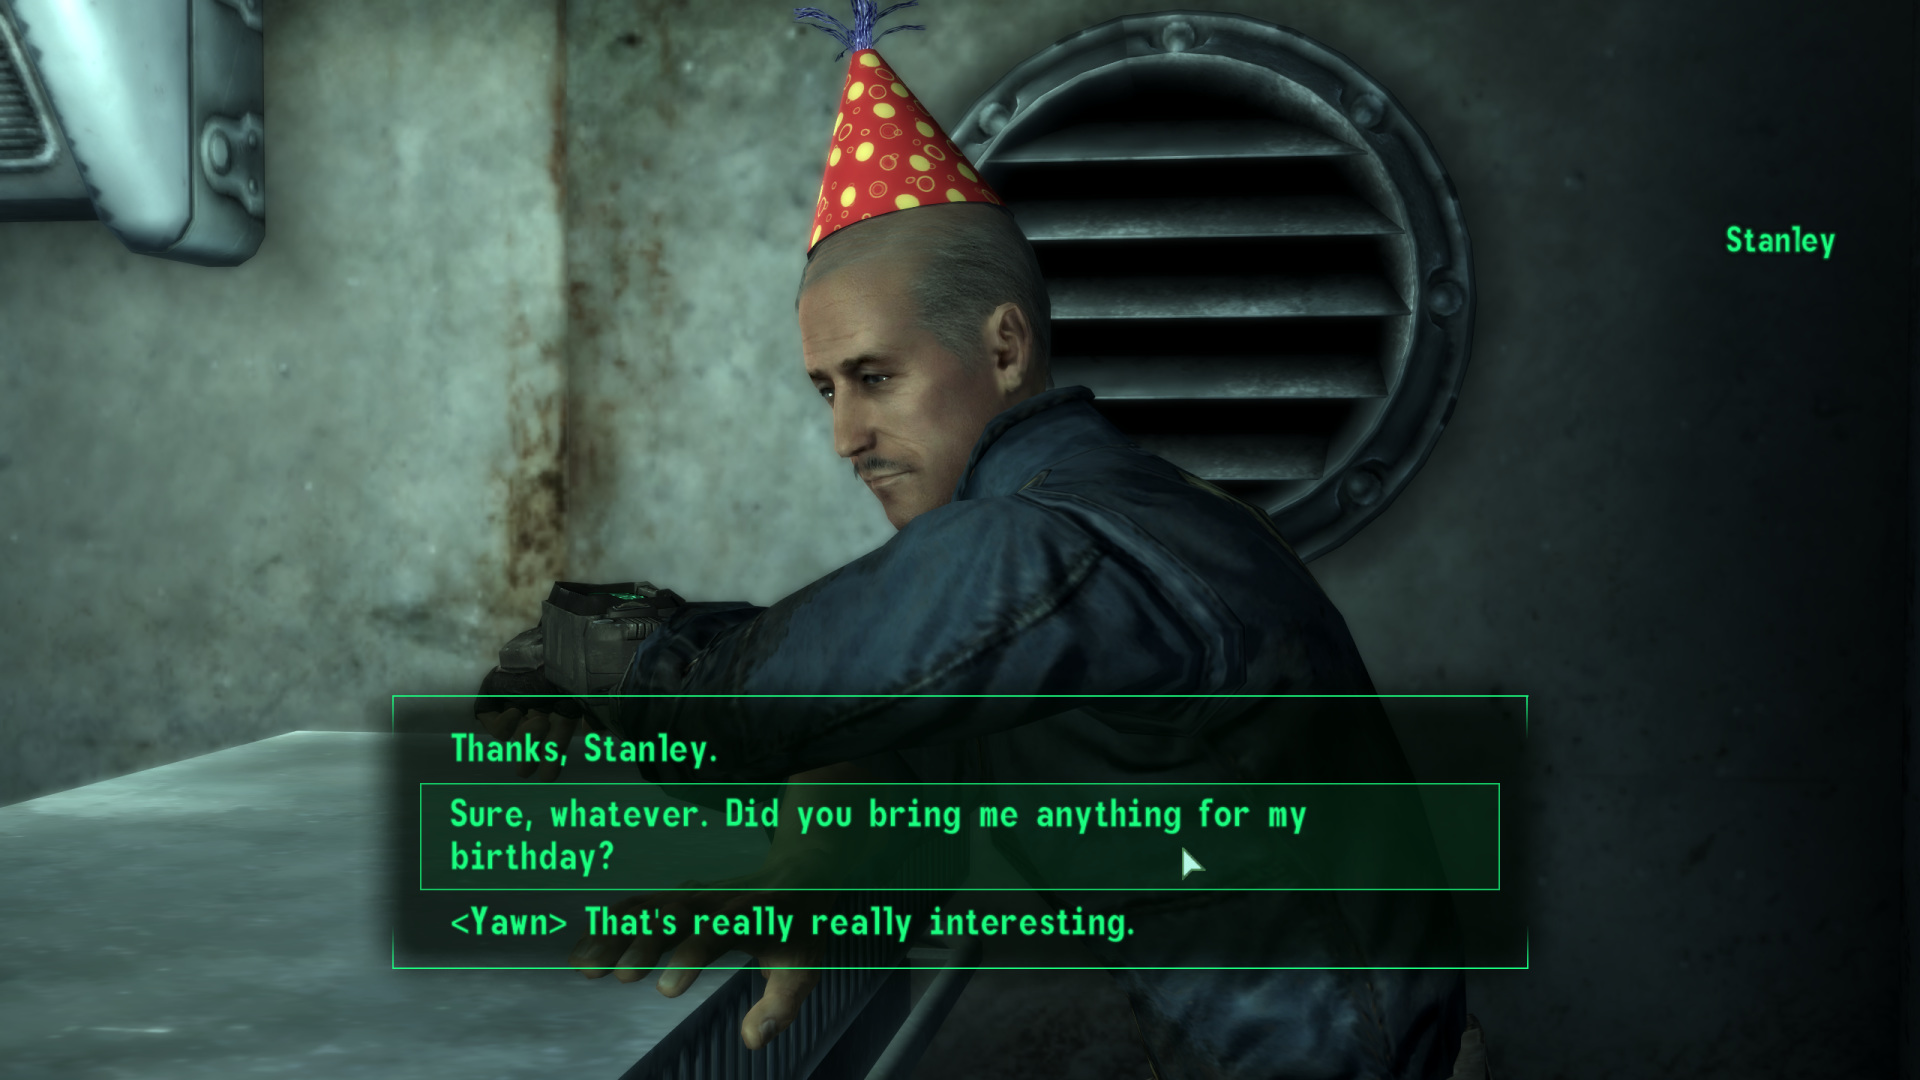
\includegraphics[width=0.8\textwidth]{images/fallout3}
\caption[Kadr z gry \textit{Fallout 3} przedstawiający przykładowy dialog.]{Kadr z gry \textit{Fallout 3} przedstawiający przykładowy dialog\protect\footnotemark.}
\label{fig:fallout}
\end{figure}
\footnotetext{Internet, \url{https://www.gameuidatabase.com/uploads/Fallout-307252021-055357-81413.jpg}, dostęp: 12.09.2023}
